% Infografía: el problema del inversor con activos en varias plataformas, con las
% frecuencias de la encuesta (N=190, muestra de conveniencia; ver Anexo C).
\begin{figure}[ht]\centering
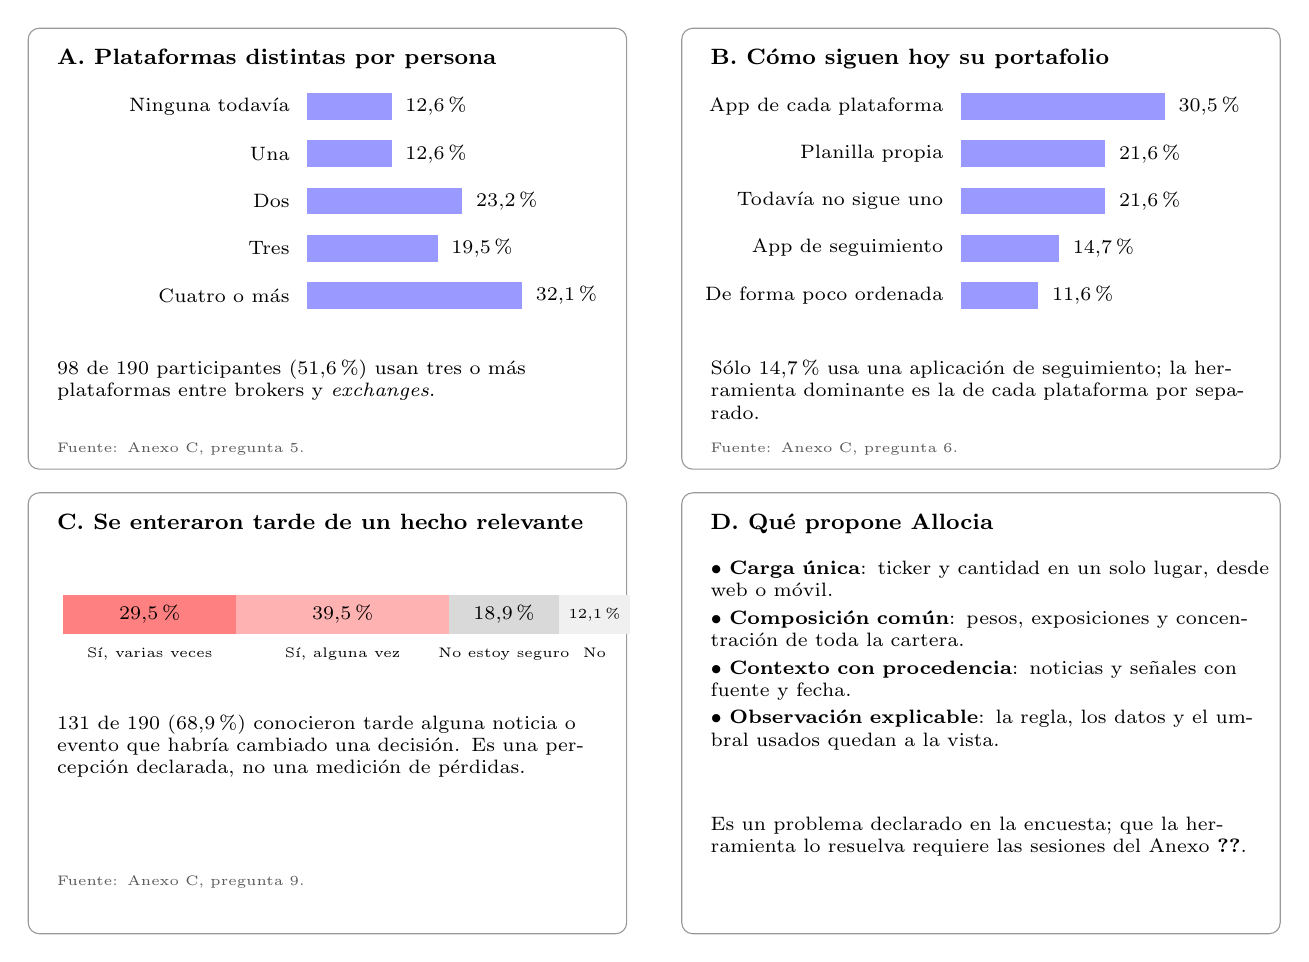
\begin{tikzpicture}[font=\scriptsize,
  panel/.style={draw=black!40,rounded corners,fill=white,minimum width=7.6cm,minimum height=5.6cm,anchor=north west},
  ttl/.style={font=\footnotesize\bfseries,anchor=north west},
  lab/.style={anchor=east,text width=3.2cm,align=right,font=\scriptsize},
  val/.style={anchor=west,font=\scriptsize},
  par/.style={anchor=north west,text width=7.1cm},
  src/.style={anchor=south west,font=\tiny,text=black!65,text width=7.1cm}]
%% Panel A: plataformas
\node[panel] at (0,0) {};
\node[ttl] at (0.25,-0.15) {A. Plataformas distintas por persona};
\begin{scope}[shift={(0.25,0)}]
\foreach \y/\n/\v/\t in {-1.0/Ninguna todavía/12.6/12{,}6, -1.6/Una/12.6/12{,}6, -2.2/Dos/23.2/23{,}2, -2.8/Tres/19.5/19{,}5, -3.4/Cuatro o más/32.1/32{,}1}{
  \node[lab] at (3.2,\y) {\n};\fill[blue!40] (3.3,\y-0.17) rectangle ({3.3+\v*0.085},\y+0.17);\node[val] at ({3.35+\v*0.085},\y) {\t\,\%};}
\end{scope}
\node[par] at (0.25,-4.1) {98 de 190 participantes (51{,}6\,\%) usan tres o más plataformas entre brokers y \textit{exchanges}.};
\node[src] at (0.25,-5.55) {Fuente: Anexo C, pregunta 5.};
%% Panel B: seguimiento
\node[panel] at (8.3,0) {};
\node[ttl] at (8.55,-0.15) {B. Cómo siguen hoy su portafolio};
\begin{scope}[shift={(8.55,0)}]
\foreach \y/\n/\v/\t in {-1.0/App de cada plataforma/30.5/30{,}5, -1.6/Planilla propia/21.6/21{,}6, -2.2/Todavía no sigue uno/21.6/21{,}6, -2.8/App de seguimiento/14.7/14{,}7, -3.4/De forma poco ordenada/11.6/11{,}6}{
  \node[lab] at (3.2,\y) {\n};\fill[blue!40] (3.3,\y-0.17) rectangle ({3.3+\v*0.085},\y+0.17);\node[val] at ({3.35+\v*0.085},\y) {\t\,\%};}
\end{scope}
\node[par] at (8.55,-4.1) {Sólo 14{,}7\,\% usa una aplicación de seguimiento; la herramienta dominante es la de cada plataforma por separado.};
\node[src] at (8.55,-5.55) {Fuente: Anexo C, pregunta 6.};
%% Panel C: enterarse tarde
\node[panel] at (0,-5.9) {};
\node[ttl] at (0.25,-6.05) {C. Se enteraron tarde de un hecho relevante};
\begin{scope}[shift={(0.25,-5.9)}]
\fill[red!50] (0.2,-1.3) rectangle (2.4,-1.8);\node[font=\scriptsize] at (1.3,-1.55) {29{,}5\,\%};
\fill[red!30] (2.4,-1.3) rectangle (5.1,-1.8);\node[font=\scriptsize] at (3.75,-1.55) {39{,}5\,\%};
\fill[black!15] (5.1,-1.3) rectangle (6.5,-1.8);\node[font=\scriptsize] at (5.8,-1.55) {18{,}9\,\%};
\fill[black!6] (6.5,-1.3) rectangle (7.4,-1.8);\node[font=\tiny] at (6.95,-1.55) {12{,}1\,\%};
\node[font=\tiny,anchor=north] at (1.3,-1.85) {Sí, varias veces};
\node[font=\tiny,anchor=north] at (3.75,-1.85) {Sí, alguna vez};
\node[font=\tiny,anchor=north] at (5.8,-1.85) {No estoy seguro};
\node[font=\tiny,anchor=north] at (6.95,-1.85) {No};
\end{scope}
\node[par] at (0.25,-8.6) {131 de 190 (68{,}9\,\%) conocieron tarde alguna noticia o evento que habría cambiado una decisión. Es una percepción declarada, no una medición de pérdidas.};
\node[src] at (0.25,-11.05) {Fuente: Anexo C, pregunta 9.};
%% Panel D: respuesta de diseño
\node[panel] at (8.3,-5.9) {};
\node[ttl] at (8.55,-6.05) {D. Qué propone Allocia};
\node[par] at (8.55,-6.65) {$\bullet$ \textbf{Carga única}: ticker y cantidad en un solo lugar, desde web o móvil.\\[2pt]
$\bullet$ \textbf{Composición común}: pesos, exposiciones y concentración de toda la cartera.\\[2pt]
$\bullet$ \textbf{Contexto con procedencia}: noticias y señales con fuente y fecha.\\[2pt]
$\bullet$ \textbf{Observación explicable}: la regla, los datos y el umbral usados quedan a la vista.};
\node[par] at (8.55,-9.9) {Es un problema declarado en la encuesta; que la herramienta lo resuelva requiere las sesiones del Anexo~\ref{annex:protocolo-usuarios}.};
\end{tikzpicture}
\caption{El problema del inversor con activos en varias plataformas según la encuesta (N=190). Fuente: elaboración propia.}\label{fig:problema-cifras}
\end{figure}
